\section{Simulation Results}
\label{s:SRTC}
The simulation results in this section simulate five different tractors transitioning into the traction control mode from open-loop commands on a firmer terrain to a lower traction terrain. A two dimensional plot of the lateral and longitudinal tractor position is shown in Fig. \ref{fig:5Tractors_2DPlot_CM2} for the five tractors colored magenta, cyan, green, blue, and red. All tractors are able to maintain tractor mobility using the traction control mode architecture except the red tractor which becomes immobilized $\sim$53 meters into the 100 meter soft terrain stretch ranging from 30 meters to 130 meters in the east position. Figure \ref{fig:5tractors_TC_traj} shows the trajectories of all 5 tractors for the east or lateral position $X$, tractor speed $v_T$, engine speed in RPM $\Omega_E$, selected gear ratio $g_{GR}$, slip ratio $i$, and throttle input $\Pi$. Table \ref{table:soft_terrain_5tractors_TC} and Fig. \ref{fig:Net_Traction_With_Payload_TC_Both} list terrain parameters for soft terrain patches for all tractors and plot net traction curves accounting for drawbar load. This is done by solving for the drawbar load at all slip values
\begin{equation}
    DB = \Bigg( \frac{F_{net}}{m_T} + \frac{R_{SD}}{m_{SD}}\Bigg)  \Bigg( \frac{m_Tm_{SD}}{mT+m_{SD}} \Bigg)
\end{equation}
and then the net traction accounting for drawbar load is given by 
\begin{equation*}
    F_{net,DB} = F_{net} - DB
\end{equation*}
This is done rearranging the equations from section \ref{s:Winch_Model_Derivation} for the dynamics in phase 2.
\begin{figure}[htbp]
    \centering
    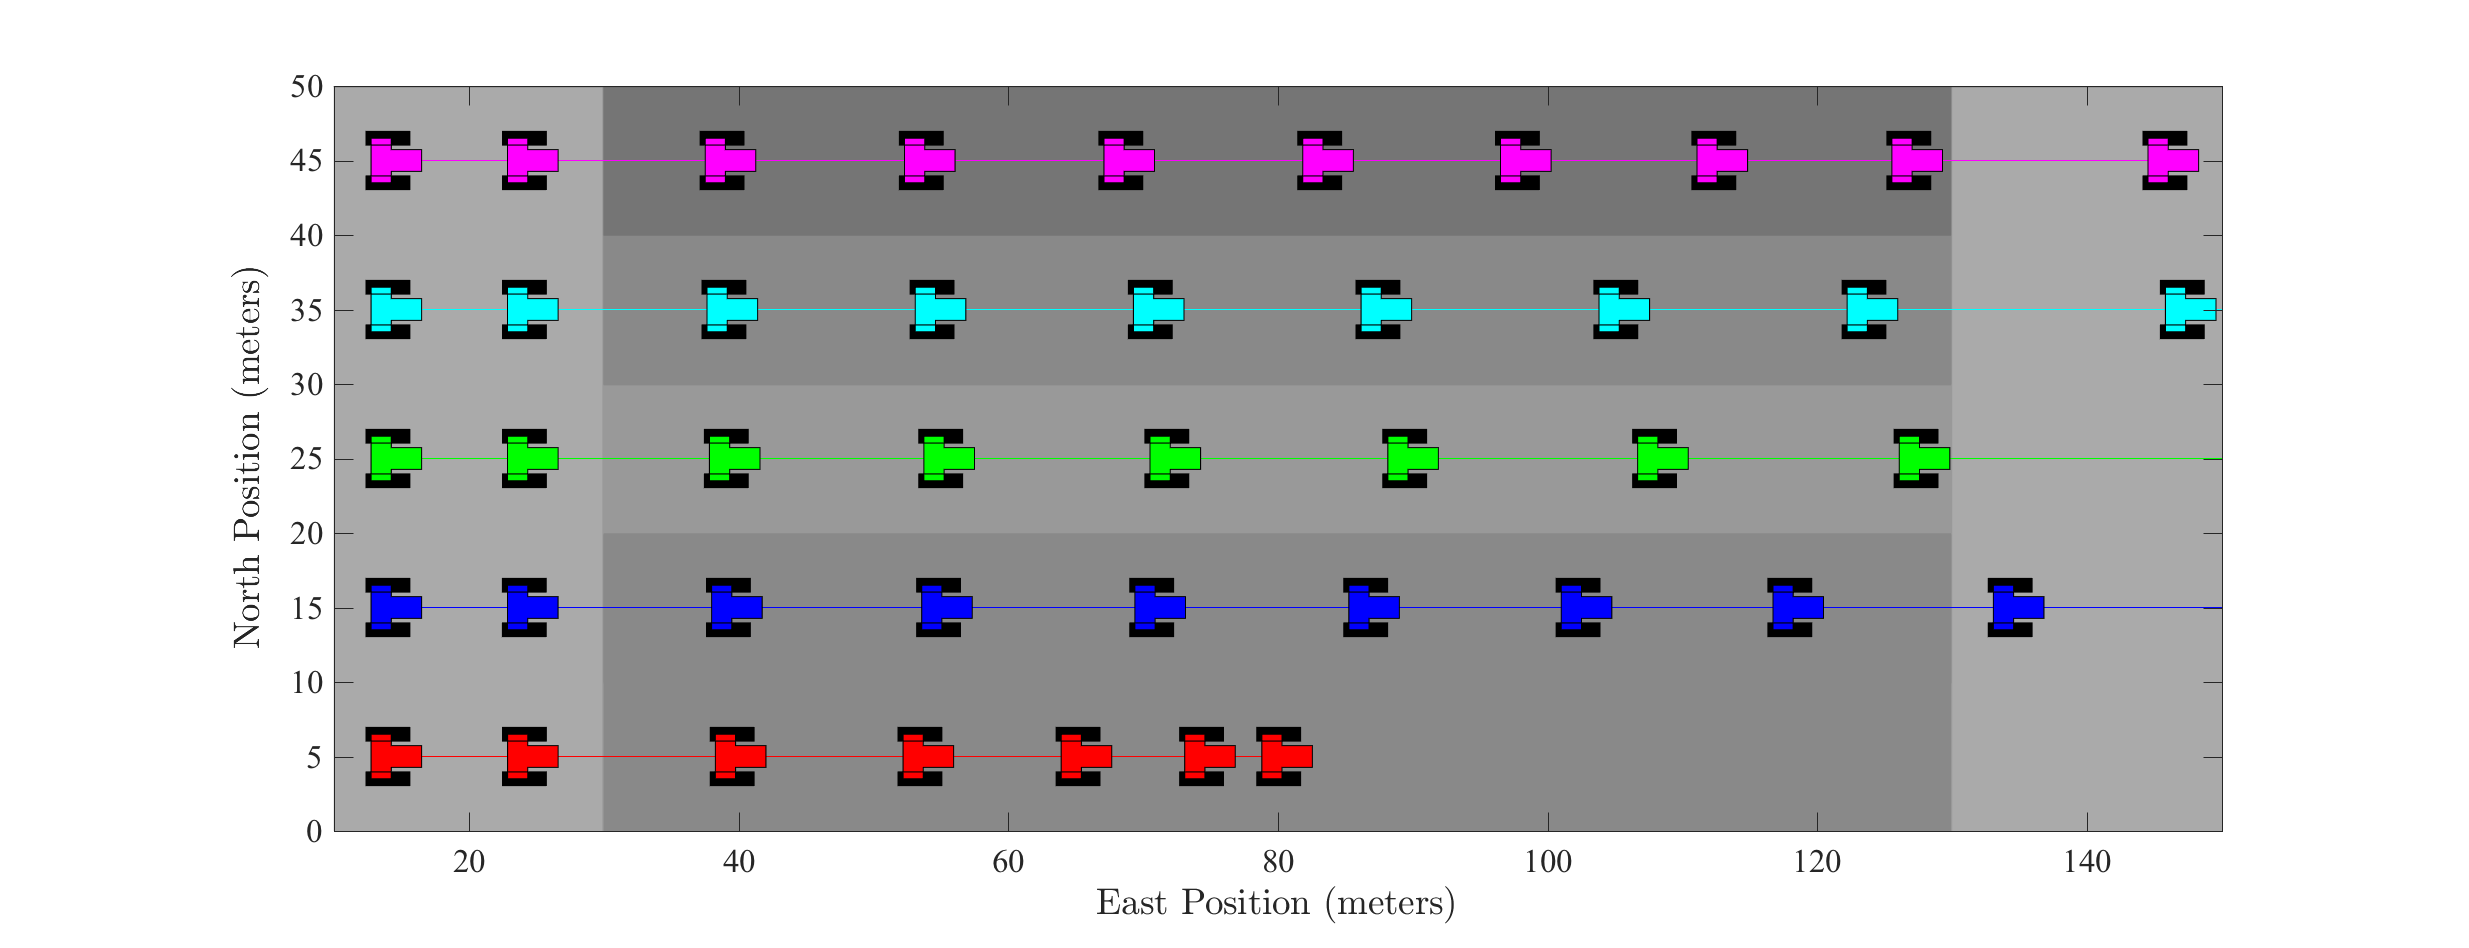
\includegraphics[width = 6.2in, keepaspectratio]{5Tractors_2DPlot_CM2}
    \caption{Two dimensional plot of north and east tractor position for five tractors colored magenta, cyan, green, blue, and red. All tractors are able to navigate the soft terrain stretch from 30 meters to 130 meters in the east coordinate using the traction control mode architecture except the red tractor.}
    \label{fig:5Tractors_2DPlot_CM2}
\end{figure}
\begin{figure}[tp]
\begin{subfigure}{0.5\textwidth}
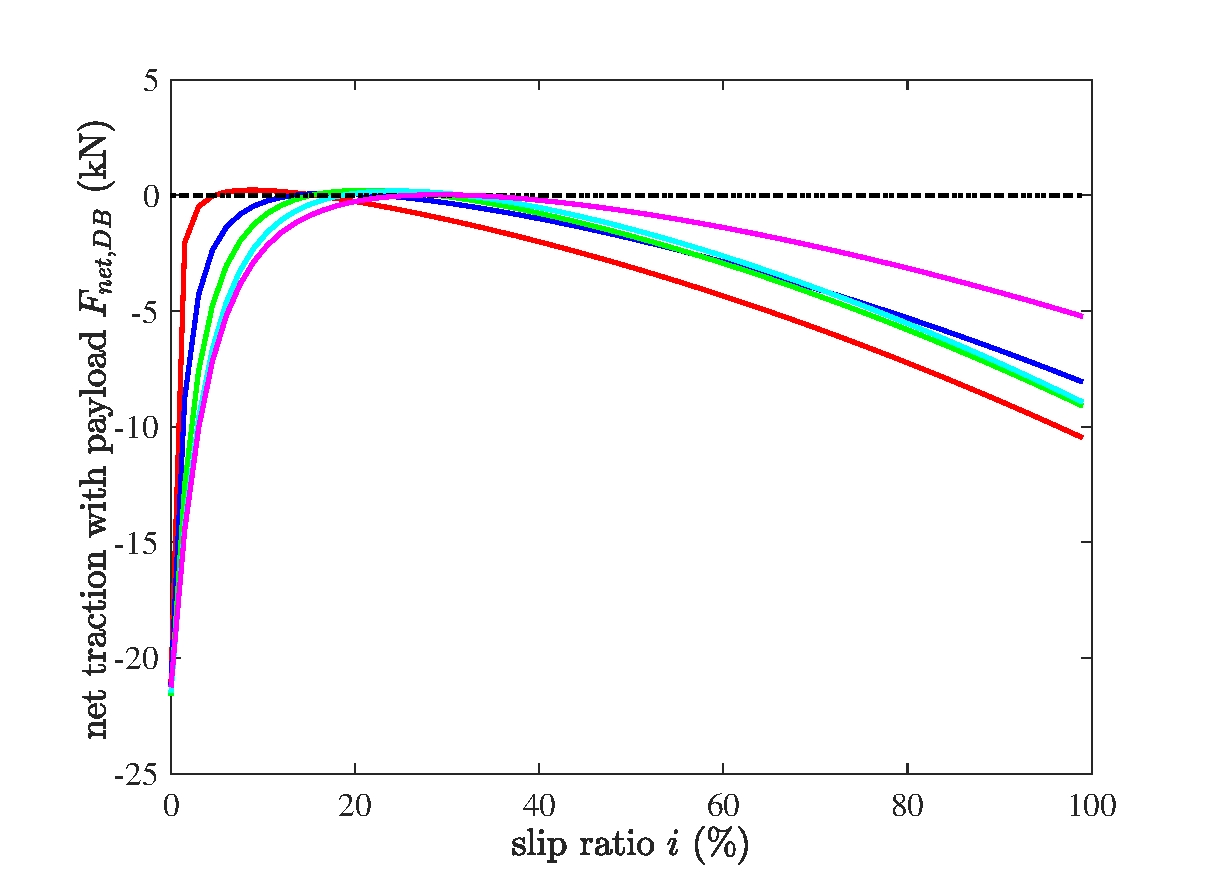
\includegraphics[width = 3.2in, keepaspectratio]{Net_Traction_With_Payload_TC}
\caption{}
\label{fig:Net_Traction_With_Payload_TC}
\end{subfigure}
\begin{subfigure}{0.5\textwidth}
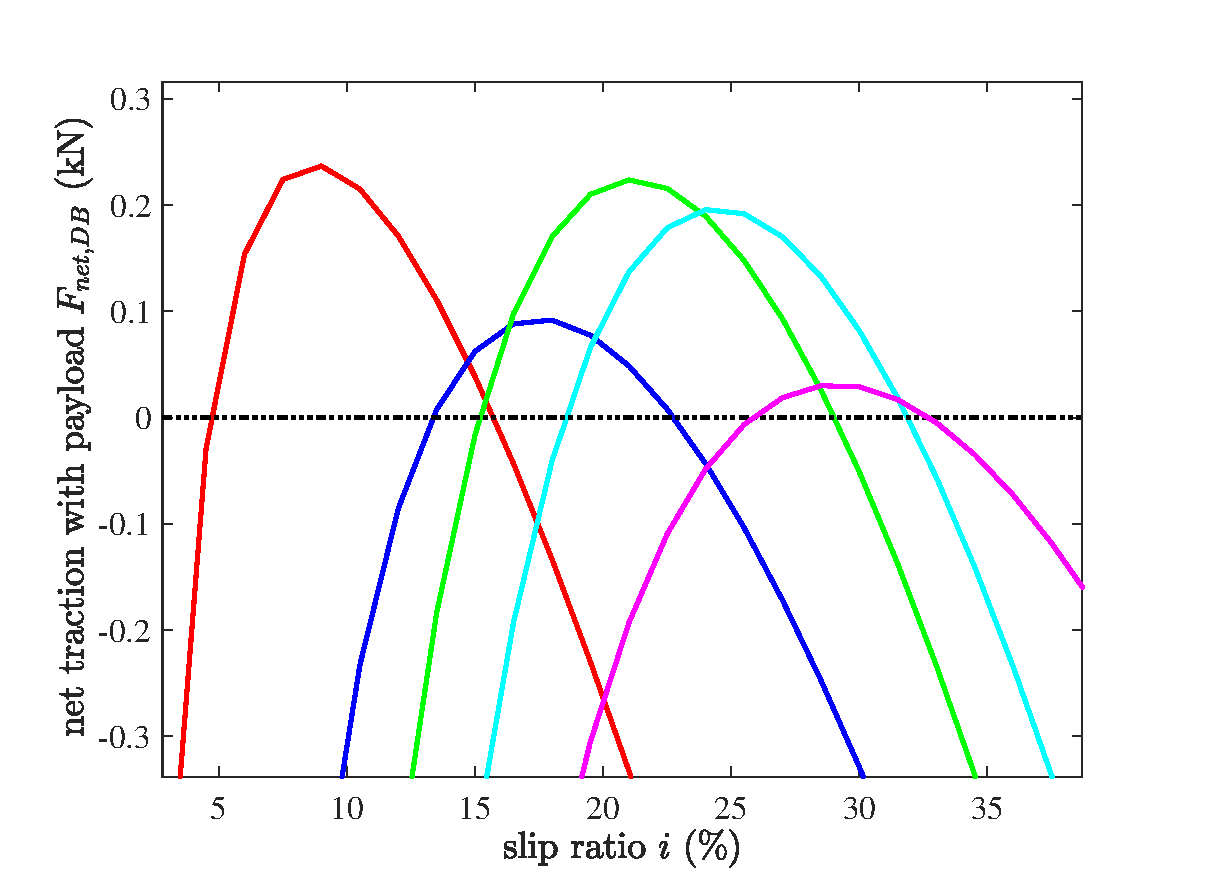
\includegraphics[width = 3.2in, keepaspectratio]{Net_Traction_With_Payload_TC_zoom}
\caption{}
\label{fig:Net_Traction_With_Payload_TC_zoom}
\end{subfigure}
\caption{(a) Net traction accouting for drawbar load $F_{net,DB}$. Colors of the $i$, $F_{net,DB}$ curves match tractor colors and the soft terrain patches they traverse shown in Fig. \ref{fig:5Tractors_2DPlot_CM2} where specific terrain paramters are given in Table \ref{table:soft_terrain_5tractors_TC}. (b) Zoomed in view of from Fig. \ref{fig:Net_Traction_With_Payload_TC} showing the small domain of $i$ yielding positive $F_{net,DB}$ values. }
\label{fig:Net_Traction_With_Payload_TC_Both}
\end{figure}
\begin{table}[tp]
\caption{Soft terrain parameters for each of the five tractors}
\label{table:soft_terrain_5tractors_TC}
\begin{center}
\vspace{-5mm}
\begin{tabular}{ |c|c|c|c|c|c|c| } 
 \hline
 tractor color & $c$ & $\Phi$ & $n$ & $k_{eq}$ & $K$ & $S$ \\ 
 \hline
  \vspace{-0.6mm} & \vspace{-0.6mm} & \vspace{-0.6mm} & \vspace{-0.6mm} & \vspace{-0.6mm} & \vspace{-0.6mm} & \vspace{-0.6mm}  \\
 \hline
 magenta & $6.1\hspace{1mm}kPa$ & $15.3^o$ & $1$ & $490\hspace{1mm}(kN/m^{n+2})$ & $7\hspace{1mm}cm$ & $80\%/33\%$\\ 
 \hline
 cyan & $5.7\hspace{1mm}kPa$ & $16.8^o$ & $1$ & $375\hspace{1mm}(kN/m^{n+2})$ & $6.8\hspace{1mm}cm$ & $ 90\%/33\%$ \\ 
 \hline
 green & $4.3\hspace{1mm}kPa$ & $18.15^o$ & $1$ & $320\hspace{1mm}(kN/m^{n+2})$ & $4.9\hspace{1mm}cm$ & $80\%/33\%$ \\ 
 \hline
 blue & $3.9\hspace{1mm}kPa$ & $17.1^o$ & $1$ & $470\hspace{1mm}(kN/m^{n+2})$ & $2.7\hspace{1mm}cm$ & $90\%/33\%$ \\ 
 \hline
 red & $3\hspace{1mm}kPa$ & $17.8^o$ & $1$ & $333\hspace{1mm}(kN/m^{n+2})$ & $0.7\hspace{1mm}cm$ & $80\%/33\%$ \\ 
 \hline
\end{tabular}
\end{center}
\end{table}
The zoomed in plot in Fig. \ref{fig:Net_Traction_With_Payload_TC_zoom} highlights the narrow domain of slip values where tractors can operate with positive $F_{net,DB}$ values. The traction control mode attempts to estimate the peak slip point $\hat{i}_{pk}$ for each terrain and regulate the tractor at that slip point. Figure \ref{fig:pk_slip_max_net_traction_estimates} plots the estimated slip point $\hat{i}_{pk}$ and maximum net traction estimate $\hat{F}_{net,max}$ for each tractor. Solid colored lines are the true value and dots indicate the estimated value. Since none of the terrain parameter vectors given in Table \ref{table:soft_terrain_5tractors_TC} match any of the hypotheses, the estimated peak slip point $i_{pk}$ can not be perfectly estimated. However, the cyan and green tractors show estimates close to their true values so the traction control mode is able to
\begin{figure}[htb]
    \centering
    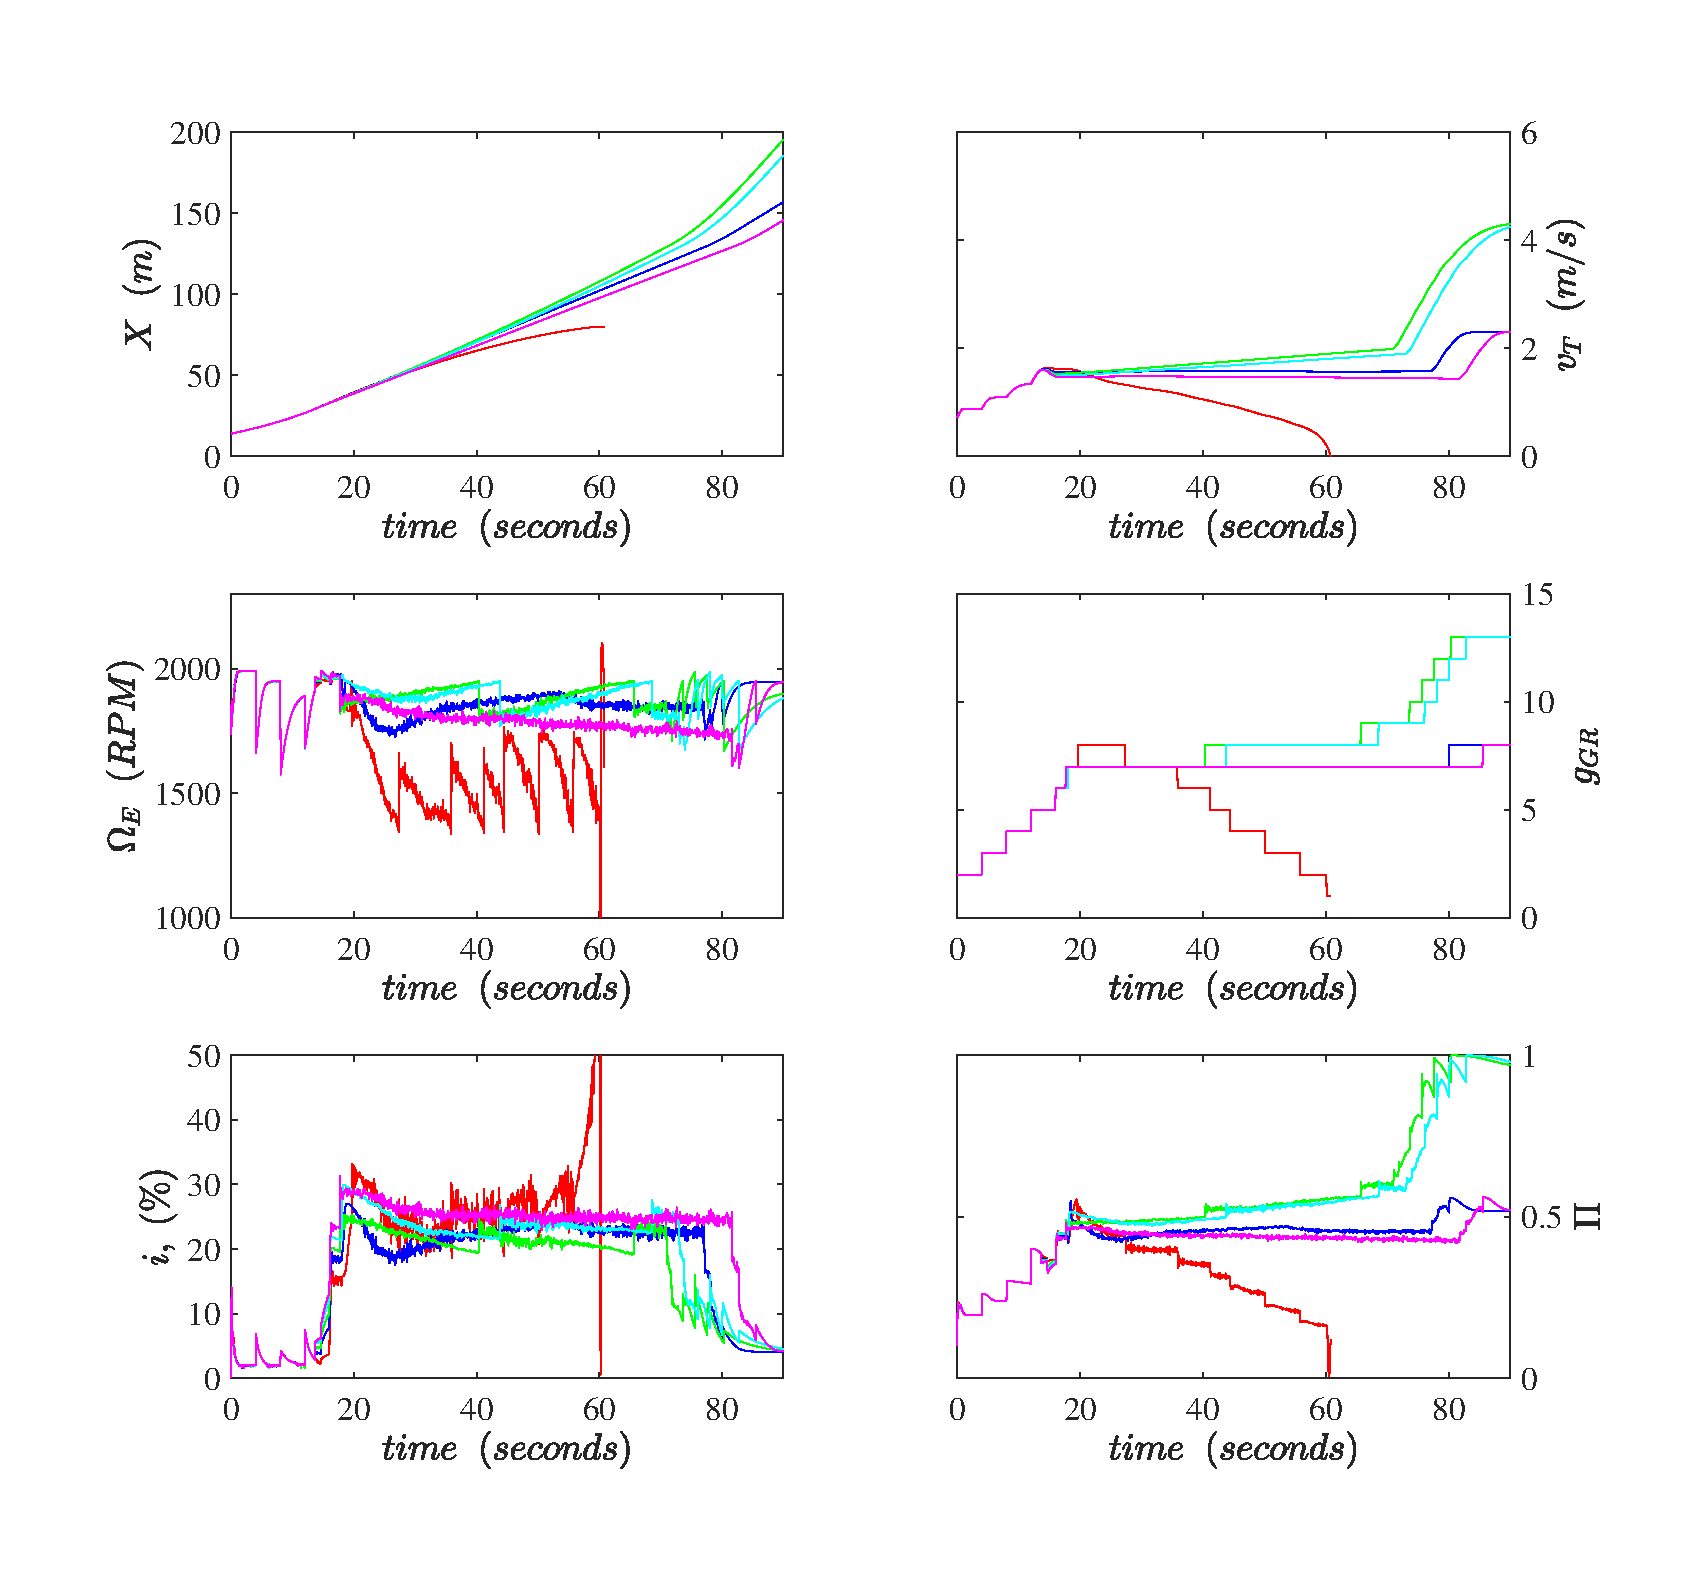
\includegraphics[height = 6in, keepaspectratio]{5tractors_TC_traj}
    \vspace{-20pt}
    \caption{Trajectories of the magenta, cyan, green, blue, and red tractors for variables of east or lateral position $X$, tractor speed $v_T$, engine speed in RPM $\Omega_E$, selected gear ratio $g_{GR}$, slip ratio $i$, and throttle input $\Pi$.}
    \label{fig:5tractors_TC_traj}
\end{figure}
\begin{figure}[htb]
    \centering
    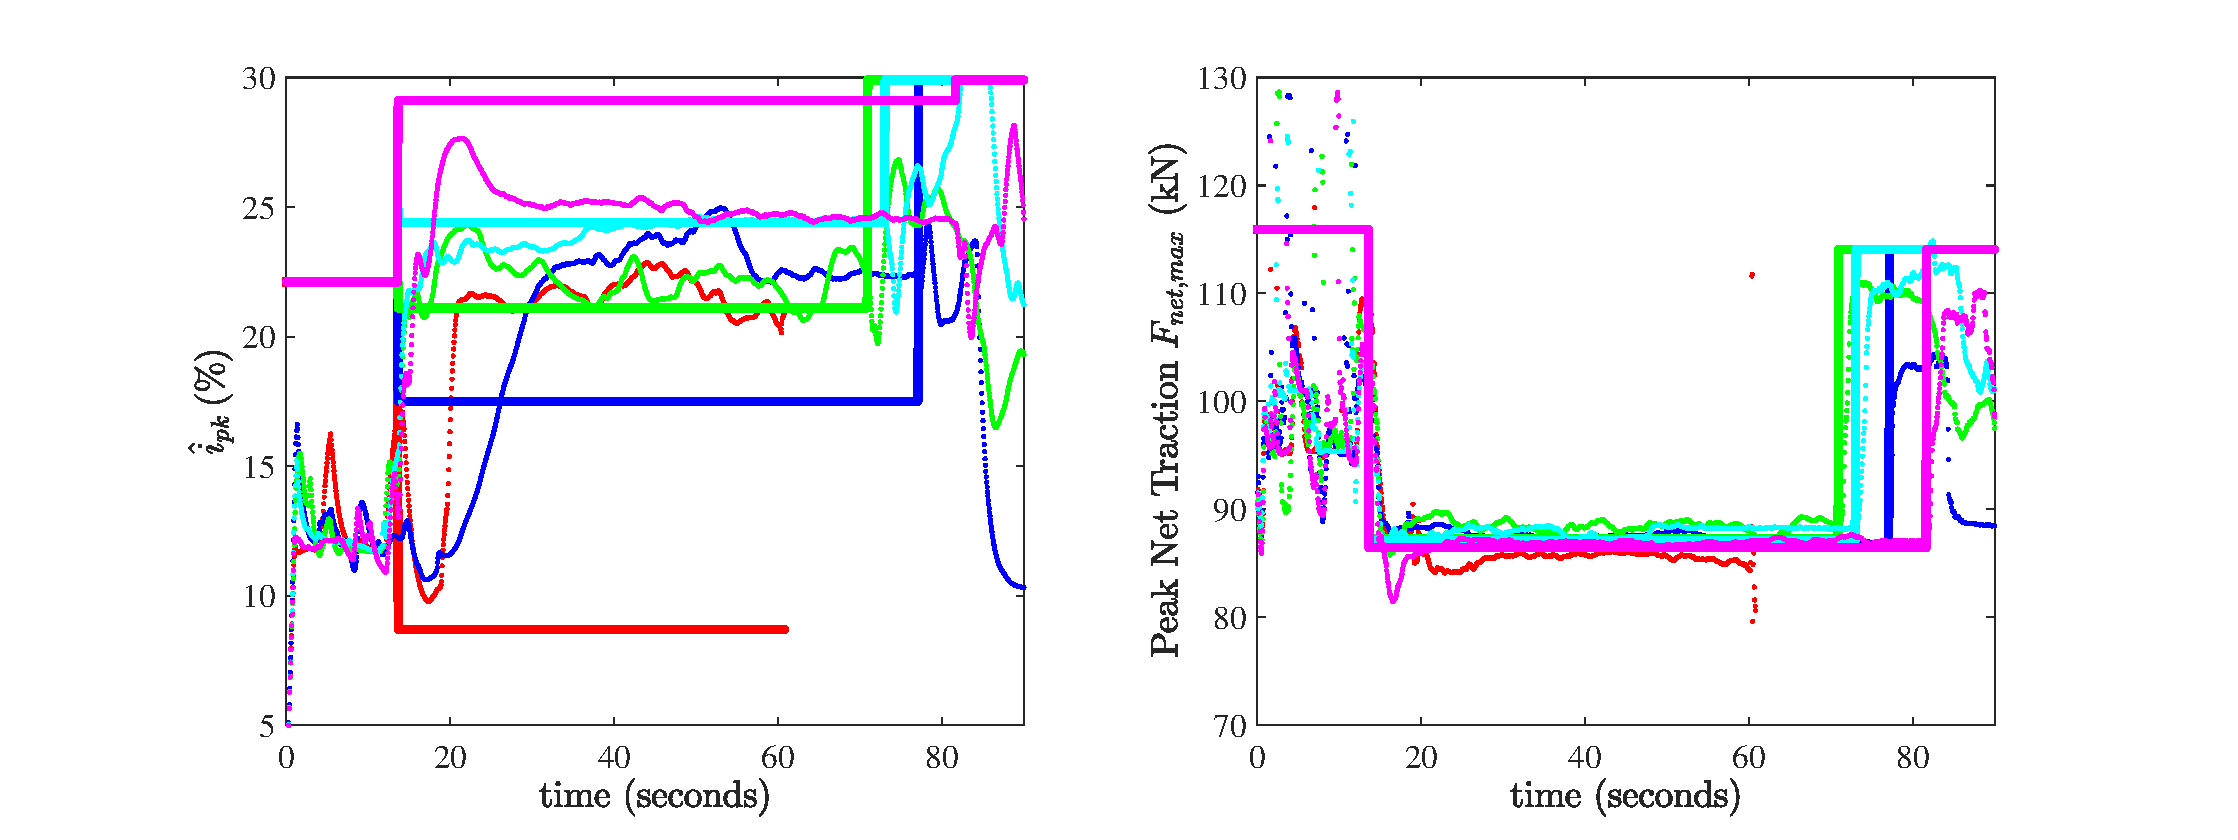
\includegraphics[width = 6.25in, keepaspectratio]{pk_slip_max_net_traction_estimates}
    \caption{Left: Estimated peak slip values $\tilde{i}_{pk}$ and true peak slip values $i_{pk}$ for all five tractors. Estimated values are denoted as dotted lines and true values are solid lines.  Right: Estimated maximum value net traction values $\hat{F}_{net}$ and true values $F_{net}$ for all five tractors. Estimated values are denoted as dotted lines and true values are solid lines. }
    \label{fig:pk_slip_max_net_traction_estimates}
\end{figure}
maintain tractor mobility and further increase ground speed across the soft terrain patch. The net traction accounting for drawbar load $F_{net,DB}$ of the magenta and blue tractors has a smaller range of slip values that provide positive net traction and smaller positive net traction values but the estimates are close enough that even though the tractors are decreasing in ground speed, they maintain mobility across the soft terrain patch. The red tractor however has a peak slip estimate $\hat{i}_{pk}$ that is significantly off and the tractor loses mobility at $\sim$ 60 seconds in the simulation. The value of $i_{pk}$ for this terrain is significantly different than the other terrains due to the very small shear deformation modulus $K=0.7\hspace{1mm}cm$ of the terrain. Once the tractor is operating under closed-loop traction control at a higher slip, determining whether or not the terrain the tractor is operating on has a high or low $K$ value is difficult since this parameter effects the shape of force slip curves at lower slip values. 
\begin{figure}[htb]
    \centering
    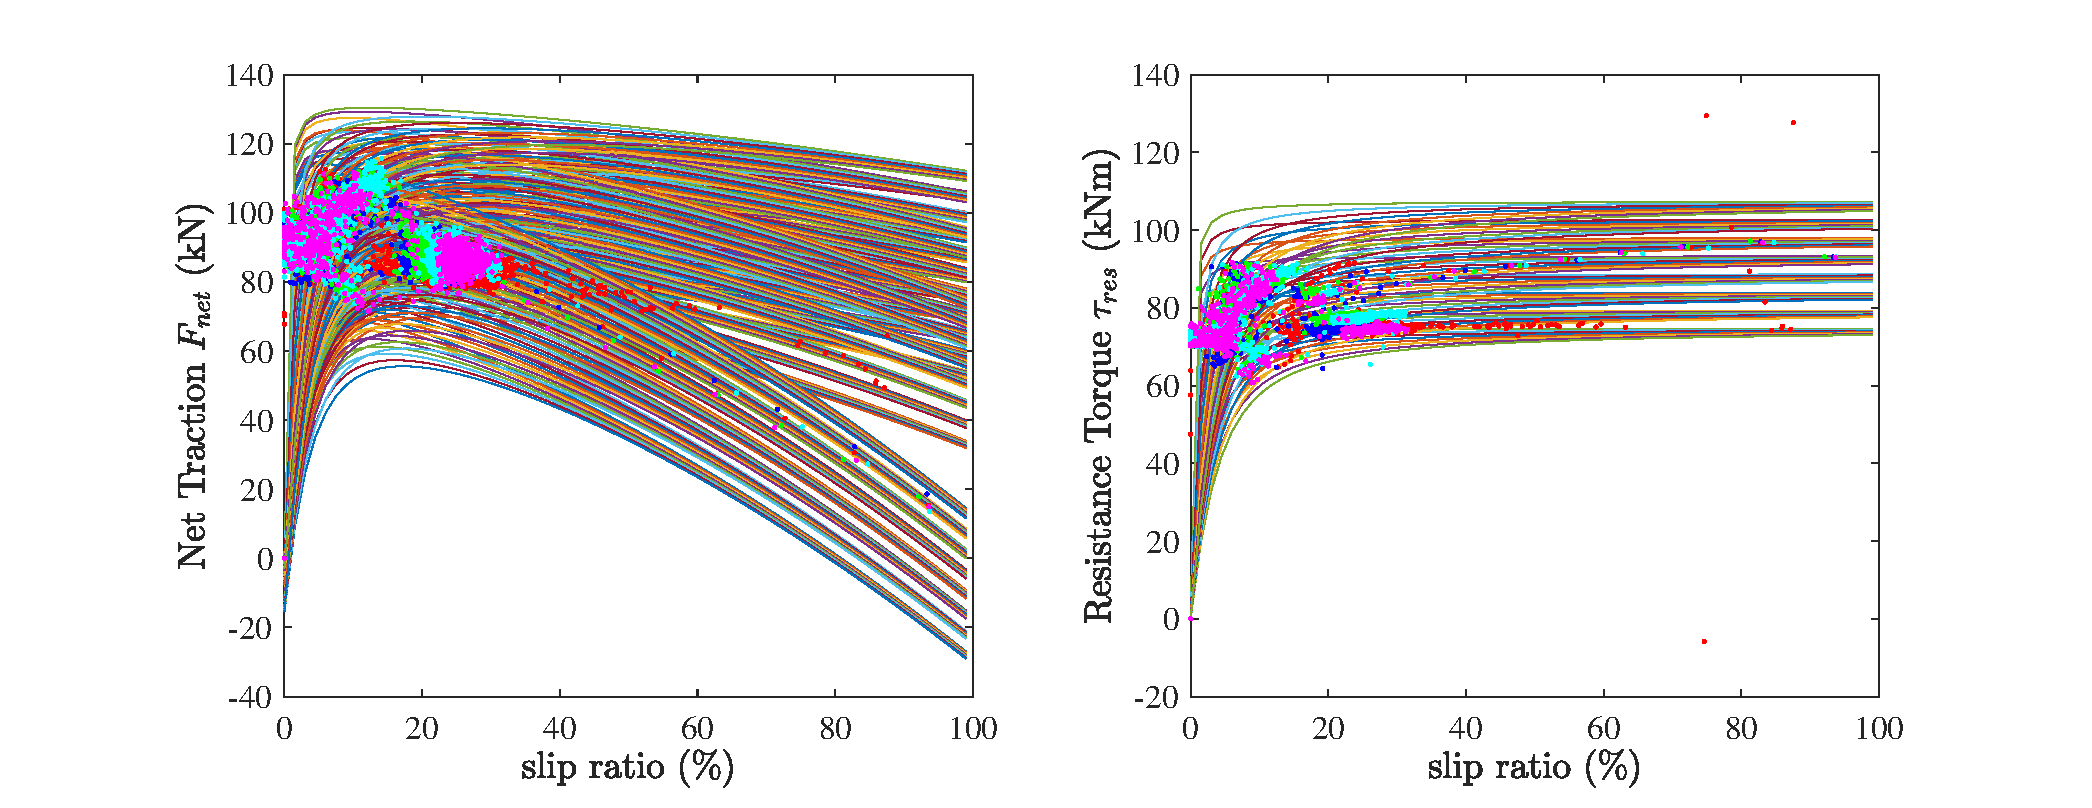
\includegraphics[width = 6in, keepaspectratio]{model_hypothesis_force_estimates}
    \caption{Terrain $[i,\hspace{1mm}F_{net}]$ and $[i,\hspace{1mm}\tau_{res}]$ slip-force curves for all 320 models based on discretization in section \ref{s:MME}. Tractor slip-force estimates are plotted as dots in the color of the respective tractor on top of the curves.}
    \label{fig:model_hypothesis_force_estimates}
\end{figure}
Figure \ref{fig:model_hypothesis_force_estimates} shows plots of the $(i,F_{net})$ and $(i,\tau_{res})$ slip force curves for all hypotheses or models considered for terrain estimation and slip force pair estimates from the DTKF that are dots whose color corresponds to tractor color. Close to all of the estimates from the DTKF under traction control are slip values of $\sim\hat{i} \geq 20 \%$. The slip force estimate clusters for both $F_{net}$ and $\tau_{res}$ for all tractors are fairly close together at approximately similar slip values. This highlights why there is difficulty at distinguishing extreme $K$ values once the tractor operates at higher slip.


